\icode{N24J-MI-SI-L2-261107-001}
\nceeID[4]{2024吉林}{3}
利用砚台将墨条研磨成墨汁时讲究“圆、缓、匀”。如图，在研磨过程中，砚台始终静止在水平桌面上。当墨条的速度方向水平向左时\paren[]

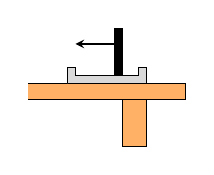
\begin{tikzpicture}[>=stealth,font=\scriptsize]
	\draw[fill=orange!60] (1,0)--(3,0)--(3,-.2)--(1,-.2) (2.2,-.2) rectangle(2.5,-.8);
	\draw[fill=gray!30] (1.5,0)--(2.5,0)--(2.5,.2)--(2.4,.2)--(2.4,.1)--(1.6,.1)--(1.6,.2)--(1.5,.2)--(1.5,0);
	\draw[fill=black] (2.1,.1) rectangle(2.2,.7);
		\draw[->] (2.1,.5)--(1.6,.5);
\end{tikzpicture}
\begin{choices}
	\item 砚台对墨条的摩擦力方向水平向左
	\item 桌面对砚台的摩擦力方向水平向左
	\item 桌面和墨条对砚台的摩擦力是一对平衡力
	\item 桌面对砚台的支持力与墨条对砚台的压力是一对平衡力
\end{choices}
\begin{answer}
    C\qquad 提示：
\end{answer}